In cui si descrive il processo di analisi della soluzione software che si intende sviluppare, enumerando i principali requisiti richiesti.

\section{Requisiti Funzionali}
I requisiti funzionali sono le funzionalità fondamentali che il sistema deve necessariamente implementare per rispondere agli obiettivi progettuali.

\subsection{Multi-tenancy}
Poiché l'obiettivo finale è la commercializzazione del prodotto sviluppato, è essenziale che il sistema supporti una gestione degli utenti basata sul modello \emph{multi-tenant}.

La gestione multi-tenant rappresenta un modello architetturale utilizzato nei sistemi software, in particolare nelle applicazioni SaaS, dove molteplici utenti (\emph{tenant}) condividono la stessa infrastruttura software e hardware. In questo contesto, i dati e le configurazioni di ciascun tenant vengono mantenuti separati e isolati, almeno a livello logico e funzionale, anche se non necessariamente a livello fisico.

Nel caso specifico di questa applicazione, la logica \emph{multi-tenant} è applicata alla gestione delle utenze del sistema. Durante l'analisi sono state identificate due possibili gerarchie di gestione degli utenti.

\subsubsection{Gerarchia a tre livelli}
\label{3-level}
In questa configurazione, la gerarchia delle utenze è strutturata come segue:

\begin{enumerate}
    \item \textbf{Utenza amministrativa principale}: posizionata al vertice della gerarchia, questa utenza ha poteri pressoché illimitati sul sistema ed è gestita esclusivamente dall'azienda responsabile del sistema stesso.
    \item \textbf{Tenant}: rappresentano rivenditori (\emph{reseller}) del servizio o entità organizzative multi individuo, come aziende o enti, che possono disporre di ulteriori clienti o utenti. Questi tenant sono creati dall'utenza amministrativa principale e possono creare utenti di livello inferiore.
    \item \textbf{Utenti semplici}: si trovano all'ultimo livello della gerarchia. Queste utenze possono essere create sia dai tenant che dall'utenza amministrativa principale, anche se quest'ultima, realisticamente, non dovrebbe aver bisogno di farlo.
\end{enumerate}

Ogni utenza può visualizzare, controllare e gestire le attività svolte dalle utenze dei livelli inferiori, ma non da quelle dello stesso livello o superiore.

Nel contesto del sistema proposto, tutti gli utenti all'interno di questa gerarchia hanno la capacità di creare e configurare task di scansione, bersagli, e consultare i risultati. Tuttavia, le funzionalità sono soggette a limitazioni basate sulle risorse assegnate. Ogni utente di livello inferiore è vincolato dai limiti imposti dall'utenza responsabile per la sua creazione (per maggiori dettagli, vedere \ref{quote-spec}).

\begin{figure}[h]
    \centering
    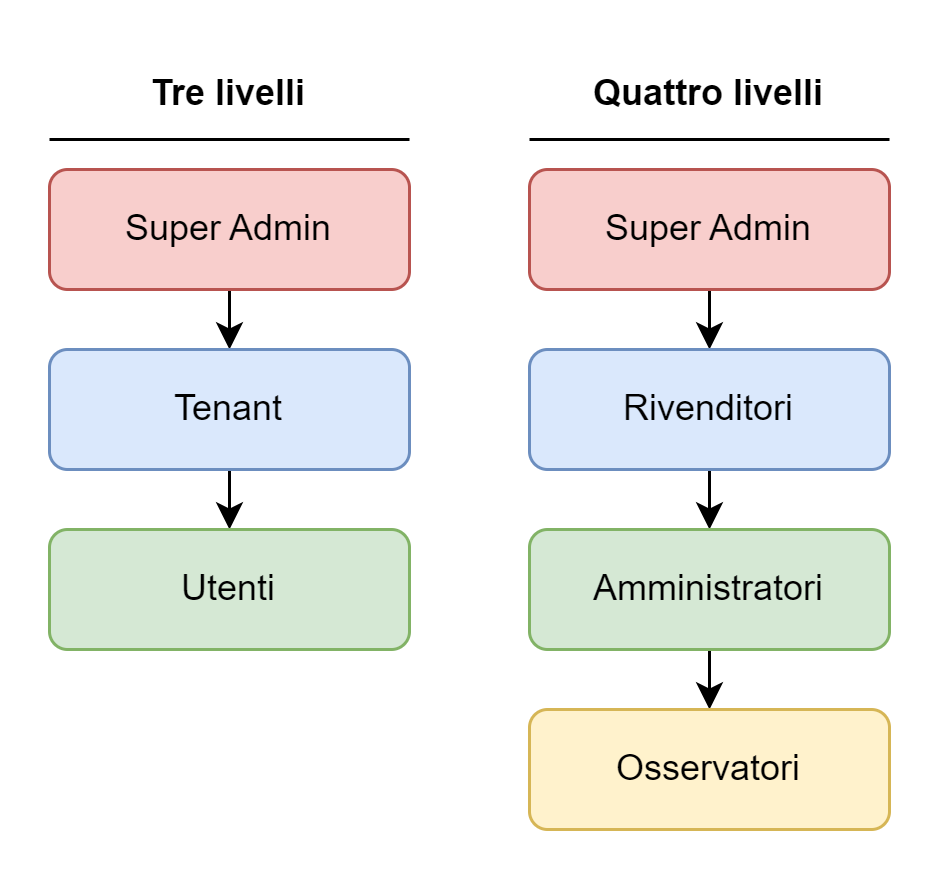
\includegraphics[width=0.6\textwidth]{img/hierarchies.png}
    \caption{Gerarchie di utenti considerate per la funzionalità di multi-tenancy}
\end{figure}

\subsubsection{Gerarchia a quattro livelli}
\label{4-level}
Un'alternativa alla precedente è rappresentata da una gerarchia a quattro livelli, strutturata come segue:

\begin{enumerate}
    \item \textbf{Utenza amministrativa principale}: posizionata al vertice, con poteri illimitati e la facoltà di creare e gestire le utenze sottostanti.
    \item \textbf{Rivenditori / \emph{Reseller}}: queste utenze rappresentano i fornitori del servizio ai clienti finali e possono creare utenti rappresentanti di tali clienti.
    \item \textbf{Clienti amministratori}: utenti che rappresentano singoli clienti privati o amministratori di sistema di aziende. Questi ultimi possono essere responsabili per la sicurezza informatica aziendale o appartenere a dipartimenti specifici, come il CED\footnote{Centro Elaborazione Dati: struttura dedicata alla gestione delle informazioni aziendali in ambito informatico.} o il SOC\footnote{Security Operations Center: centro operativo dedicato alla sicurezza informatica, con focus su risposta agli incidenti e monitoraggio preventivo delle minacce tramite strumenti specifici come SIEM, IDS o IPS.}.
    \item \textbf{Utenti aziendali}: situati all'ultimo livello, questi utenti hanno accesso limitato alle funzionalità del sistema, con la sola possibilità di monitorare e consultare i dati raccolti, senza intervenire sul processo di scansione.
\end{enumerate}

Questa architettura è simile alla precedente, con l'unica aggiunta di un ulteriore livello che consente una visione parziale dei risultati prodotti dal livello immediatamente superiore, senza però poter configurare o modificare alcun parametro del sistema.

\subsection{Limiti d'uso (quote di scansione)}
\label{quote-spec}
Poiché questo progetto è concepito per evolversi in un SaaS (come discusso in \ref{saas}), una parte cruciale del processo di analisi è stata la progettazione di un sistema di controllo delle risorse, eventualmente collegato al modello di pagamento degli utenti.

In prima istanza, è stato considerato un sistema di quote mensili per le scansioni. Una quota, in questo contesto, è definita come un numero intero maggiore di zero ($n > 0$), che indica il numero di nodi scansionabili in un mese dall'utente a cui è attribuita. In termini pratici, la quota corrisponde al numero di indirizzi IP che l'utente può sottoporre a scansione mensilmente utilizzando il servizio.

Le condizioni d'uso specifiche sono le seguenti:
\begin{itemize}
    \item Il numero di scansioni assegnato si rinnova all'inizio di ogni mese, indipendentemente dalla diversa durata dei mesi.
    \item Ogni scansione che coinvolge $n$ indirizzi IP consuma esattamente $n$ unità della quota mensile disponibile.
    \item I nodi non attivi (``spenti'') contano comunque ai fini del decremento della quota.
    \item Scansionare ripetutamente lo stesso indirizzo IP nello stesso mese comporta una riduzione della quota per ogni iterazione della scansione.
    \item Le unità di quota non consumate entro la fine del mese non sono cumulabili per i mesi successivi.
\end{itemize}

Le quote sono stabilite e assegnate dall'utente responsabile per la creazione dell'utenza interessata. Tuttavia, l'effettivo processo di fatturazione al cliente finale non rientra nell'ambito del progetto e si suppone realizzato separatamente.

\subsection{Task di scansione}
Il sistema software dovrebbe consentire la definizione di \emph{task} di scansione su nodi di rete specifici.

L'obiettivo primario di tali task è condurre un \textbf{vulnerability assessment} completo, senza includere elementi di \emph{penetration testing}, sia manuale che semi-automatico.

In aggiunta alla selezione dei bersagli, i task di scansione devono essere configurabili dall'utente per quanto riguarda il livello di dettaglio dei risultati e l'organizzazione temporale delle esecuzioni.

\subsubsection{Temporizzazione e calendarizzazione}
Il sistema deve supportare la definizione di task di scansione ricorrenti, programmabili secondo calendari a cadenza regolare, come quella mensile.

In alternativa, gli utenti devono avere la possibilità di definire task di scansione \emph{ad hoc}, da eseguire una tantum per verifiche specifiche di sicurezza su uno o più nodi.

\subsection{Bersagli}
I bersagli delle scansioni devono poter essere gestiti con la massima flessibilità. Il sistema deve supportare:
\begin{itemize}
    \item Nomi di dominio (DNS);
    \item Indirizzi IPv4 e IPv6;
    \item Insiemi di nodi o indirizzi IP, specificati attraverso notazioni come la CIDR.
\end{itemize}

Inoltre, il sistema deve consentire l'importazione di liste di bersagli tramite file esterni. Questa funzionalità è particolarmente utile in contesti aziendali, dove gli host da analizzare sono spesso numerosi e generati automaticamente da procedure interne, rendendo poco pratico l'inserimento manuale.

\subsection{Risultati}
I risultati delle scansioni devono essere facilmente consultabili, con particolare enfasi su:
\begin{itemize}
    \item La severità delle vulnerabilità rilevate;
    \item Le possibili soluzioni o mitigazioni suggerite;
    \item Altri dettagli tecnici pertinenti, raccolti durante il processo di scansione.
\end{itemize}

Il sistema deve offrire strumenti per filtrare, ordinare e gestire i risultati, garantendo una visualizzazione chiara e intuitiva delle informazioni rilevanti.

\section{Requisiti non funzionali}
Ovvero come il sistema deve comportarsi e a quali standard di qualità, prestazioni, sicurezza e usabilità dovrà conformarsi.

\subsection{Facilità d'uso}
L'interfaccia (UI) e l'esperienza utente (UX) devono essere necessariamente facili e intuitive, con il minor numero possibile di complicazioni esposte all'utente finale.

Il sistema deve pertanto integrare già di per sé dei \emph{default} sicuri e affidabili, lasciando all'utente finale la personalizzazione solo delle parti meno critiche. Il sistema dovrà anche nascondere tutti i dettagli tecnici, ove possibile, limitandosi a mostrare solo lo stretto necessario per comprendere \emph{cosa} e stato trovato e \emph{come} risolverlo (se possibile).

\subsection{Efficienza}
Il sistema deve essere necessariamente efficiente, senza rallentamenti eccessivi nella sua interfaccia. Questo diventa particolarmente critico in sede di reportistica ed analisi dei risultati, dove spesso i dati raccolti da questi sistemi possono accumularsi velocemente.

\section{Requisiti di sistema}
Ovvero quali specifiche tecniche e infrastrutturali dovranno essere rispettate dal sistema in oggetto.

\subsection{Software as a Service}
\label{saas}
Il software che si intende creare sarà a tutti gli effetti un \textbf{SaaS} (Software as a Service). In un modello SaaS, l'applicazione software è installata su uno e più server remoti e vengono fornite agli utenti finali tramite Internet. Il software non viene acquistato, installato e gestito localmente, ma accedono al software e lo usano direttamente, solitamente tramite browser web e a fronte di un abbonamento periodico.

In questo caso specifico la quota di scansione definita in \ref{quote-spec} è il privilegio che viene fornito a fronte del pagamento.

\subsection{Integrazione con scanner esistenti}
Per un componente così complesso e continuamente aggiornato non è realistico pensare di sviluppare da zero un nuovo scanner in grado di competere con le principali soluzioni commerciali. Inoltre, questi sistemi sono ovviamente delicati e critici, giustificando a maggior ragione la scelta di appoggiarsi a soluzioni più mature.

Per queste ragioni, il sistema si integrerà con almeno un altro scanner preesistente. Sarebbe preferibile avere un sistema sufficientemente flessibile da garantire l'interoperabilità con diversi backend di scansione.

Inoltre, lo scanner considerato dovrà necessariamente avere eccellenti doti di interoperabilità con altri sistemi software.

\subsection{Architettura a microservizi}
\label{microservices}
Come spiegato nella precedente sezione, il sistema in oggetto trarrebbe vantaggi dall'essere strutturato in un'architettura non monolitica. Questo sia a carattere di facilità di manutenzione, sia per velocizzare eventuali refactor a seguito di un cambio del backend.

La separazione dei componenti inoltre facilita lo sviluppo di eventuali client, in grado di appoggiarsi alle API esposte dai singoli microservizi.